\documentclass[1p]{elsarticle_modified}
%\bibliographystyle{elsarticle-num}

%\usepackage[colorlinks]{hyperref}
%\usepackage{abbrmath_seonhwa} %\Abb, \Ascr, \Acal ,\Abf, \Afrak
\usepackage{amsfonts}
\usepackage{amssymb}
\usepackage{amsmath}
\usepackage{amsthm}
\usepackage{scalefnt}
\usepackage{amsbsy}
\usepackage{kotex}
\usepackage{caption}
\usepackage{subfig}
\usepackage{color}
\usepackage{graphicx}
\usepackage{xcolor} %% white, black, red, green, blue, cyan, magenta, yellow
\usepackage{float}
\usepackage{setspace}
\usepackage{hyperref}

\usepackage{tikz}
\usetikzlibrary{arrows}

\usepackage{multirow}
\usepackage{array} % fixed length table
\usepackage{hhline}

%%%%%%%%%%%%%%%%%%%%%
\makeatletter
\renewcommand*\env@matrix[1][\arraystretch]{%
	\edef\arraystretch{#1}%
	\hskip -\arraycolsep
	\let\@ifnextchar\new@ifnextchar
	\array{*\c@MaxMatrixCols c}}
\makeatother %https://tex.stackexchange.com/questions/14071/how-can-i-increase-the-line-spacing-in-a-matrix
%%%%%%%%%%%%%%%

\usepackage[normalem]{ulem}

\newcommand{\msout}[1]{\ifmmode\text{\sout{\ensuremath{#1}}}\else\sout{#1}\fi}
%SOURCE: \msout is \stkout macro in https://tex.stackexchange.com/questions/20609/strikeout-in-math-mode

\newcommand{\cancel}[1]{
	\ifmmode
	{\color{red}\msout{#1}}
	\else
	{\color{red}\sout{#1}}
	\fi
}

\newcommand{\add}[1]{
	{\color{blue}\uwave{#1}}
}

\newcommand{\replace}[2]{
	\ifmmode
	{\color{red}\msout{#1}}{\color{blue}\uwave{#2}}
	\else
	{\color{red}\sout{#1}}{\color{blue}\uwave{#2}}
	\fi
}

\newcommand{\Sol}{\mathcal{S}} %segment
\newcommand{\D}{D} %diagram
\newcommand{\A}{\mathcal{A}} %arc


%%%%%%%%%%%%%%%%%%%%%%%%%%%%%5 test

\def\sl{\operatorname{\textup{SL}}(2,\Cbb)}
\def\psl{\operatorname{\textup{PSL}}(2,\Cbb)}
\def\quan{\mkern 1mu \triangleright \mkern 1mu}

\theoremstyle{definition}
\newtheorem{thm}{Theorem}[section]
\newtheorem{prop}[thm]{Proposition}
\newtheorem{lem}[thm]{Lemma}
\newtheorem{ques}[thm]{Question}
\newtheorem{cor}[thm]{Corollary}
\newtheorem{defn}[thm]{Definition}
\newtheorem{exam}[thm]{Example}
\newtheorem{rmk}[thm]{Remark}
\newtheorem{alg}[thm]{Algorithm}

\newcommand{\I}{\sqrt{-1}}
\begin{document}

%\begin{frontmatter}
%
%\title{Boundary parabolic representations of knots up to 8 crossings}
%
%%% Group authors per affiliation:
%\author{Yunhi Cho} 
%\address{Department of Mathematics, University of Seoul, Seoul, Korea}
%\ead{yhcho@uos.ac.kr}
%
%
%\author{Seonhwa Kim} %\fnref{s_kim}}
%\address{Center for Geometry and Physics, Institute for Basic Science, Pohang, 37673, Korea}
%\ead{ryeona17@ibs.re.kr}
%
%\author{Hyuk Kim}
%\address{Department of Mathematical Sciences, Seoul National University, Seoul 08826, Korea}
%\ead{hyukkim@snu.ac.kr}
%
%\author{Seokbeom Yoon}
%\address{Department of Mathematical Sciences, Seoul National University, Seoul, 08826,  Korea}
%\ead{sbyoon15@snu.ac.kr}
%
%\begin{abstract}
%We find all boundary parabolic representation of knots up to 8 crossings.
%
%\end{abstract}
%\begin{keyword}
%    \MSC[2010] 57M25 
%\end{keyword}
%
%\end{frontmatter}

%\linenumbers
%\tableofcontents
%
\newcommand\colored[1]{\textcolor{white}{\rule[-0.35ex]{0.8em}{1.4ex}}\kern-0.8em\color{red} #1}%
%\newcommand\colored[1]{\textcolor{white}{ #1}\kern-2.17ex	\textcolor{white}{ #1}\kern-1.81ex	\textcolor{white}{ #1}\kern-2.15ex\color{red}#1	}

{\Large $\underline{11a_{275}~(K11a_{275})}$}

\setlength{\tabcolsep}{10pt}
\renewcommand{\arraystretch}{1.6}
\vspace{1cm}\begin{tabular}{m{100pt}>{\centering\arraybackslash}m{274pt}}
\multirow{5}{120pt}{
	\centering
	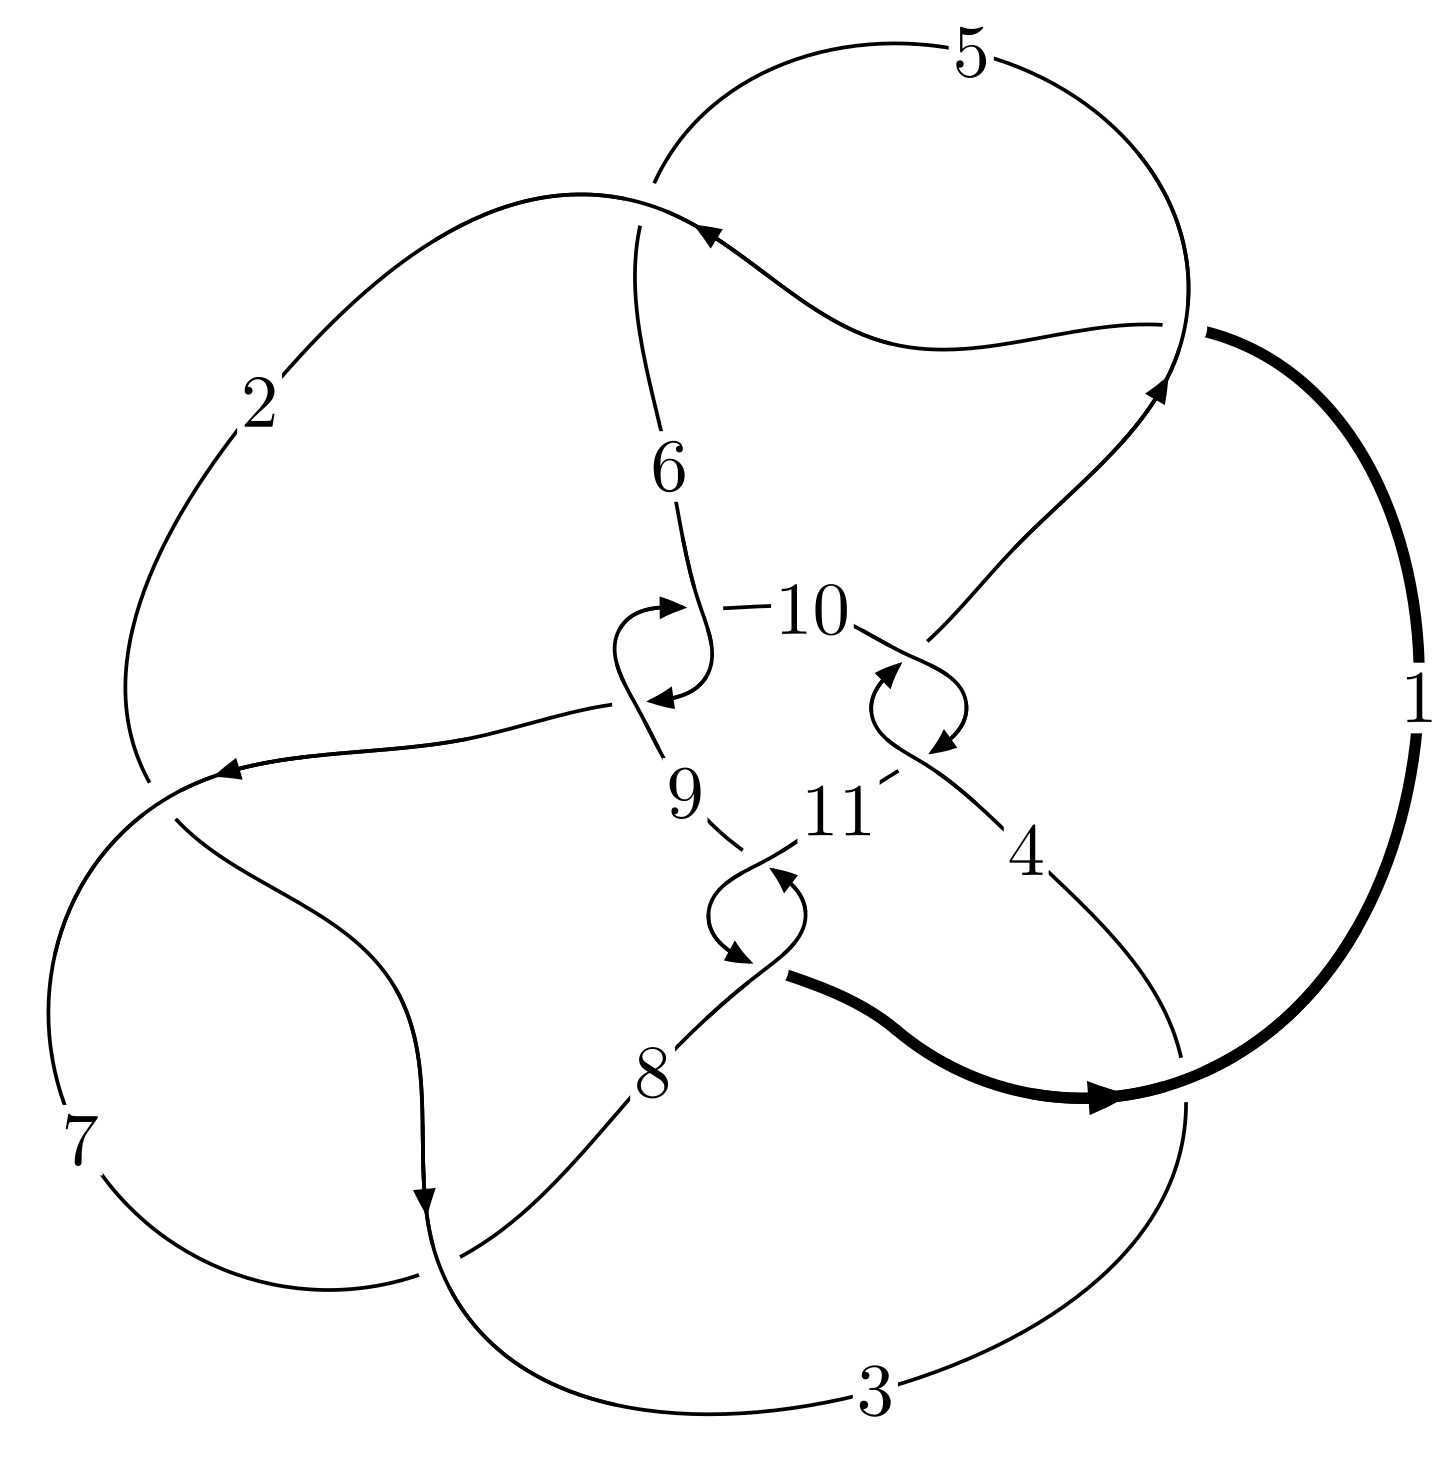
\includegraphics[width=112pt]{../../../GIT/diagram.site/Diagrams/png/524_11a_275.png}\\
\ \ \ A knot diagram\footnotemark}&
\allowdisplaybreaks
\textbf{Linearized knot diagam} \\
\cline{2-2}
 &
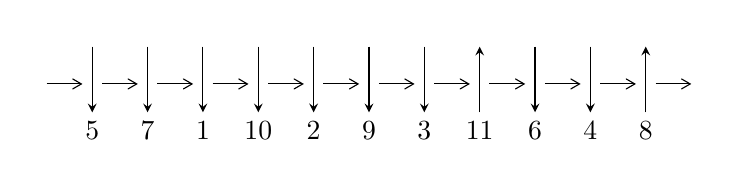
\begin{tikzpicture}[x=20pt, y=17pt]
	% nodes
	\node (C0) at (0, 0) {};
	\node (C1) at (1, 0) {};
	\node (C1U) at (1, +1) {};
	\node (C1D) at (1, -1) {5};

	\node (C2) at (2, 0) {};
	\node (C2U) at (2, +1) {};
	\node (C2D) at (2, -1) {7};

	\node (C3) at (3, 0) {};
	\node (C3U) at (3, +1) {};
	\node (C3D) at (3, -1) {1};

	\node (C4) at (4, 0) {};
	\node (C4U) at (4, +1) {};
	\node (C4D) at (4, -1) {10};

	\node (C5) at (5, 0) {};
	\node (C5U) at (5, +1) {};
	\node (C5D) at (5, -1) {2};

	\node (C6) at (6, 0) {};
	\node (C6U) at (6, +1) {};
	\node (C6D) at (6, -1) {9};

	\node (C7) at (7, 0) {};
	\node (C7U) at (7, +1) {};
	\node (C7D) at (7, -1) {3};

	\node (C8) at (8, 0) {};
	\node (C8U) at (8, +1) {};
	\node (C8D) at (8, -1) {11};

	\node (C9) at (9, 0) {};
	\node (C9U) at (9, +1) {};
	\node (C9D) at (9, -1) {6};

	\node (C10) at (10, 0) {};
	\node (C10U) at (10, +1) {};
	\node (C10D) at (10, -1) {4};

	\node (C11) at (11, 0) {};
	\node (C11U) at (11, +1) {};
	\node (C11D) at (11, -1) {8};
	\node (C12) at (12, 0) {};

	% arrows
	\draw[->,>={angle 60}]
	(C0) edge (C1) (C1) edge (C2) (C2) edge (C3) (C3) edge (C4) (C4) edge (C5) (C5) edge (C6) (C6) edge (C7) (C7) edge (C8) (C8) edge (C9) (C9) edge (C10) (C10) edge (C11) (C11) edge (C12) ;	\draw[->,>=stealth]
	(C1U) edge (C1D) (C2U) edge (C2D) (C3U) edge (C3D) (C4U) edge (C4D) (C5U) edge (C5D) (C6U) edge (C6D) (C7U) edge (C7D) (C8D) edge (C8U) (C9U) edge (C9D) (C10U) edge (C10D) (C11D) edge (C11U) ;
	\end{tikzpicture} \\
\hhline{~~} \\& 
\textbf{Solving Sequence} \\ \cline{2-2} 
 &
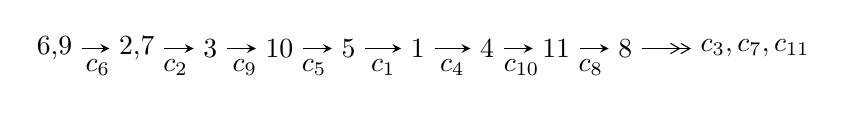
\begin{tikzpicture}[x=25pt, y=7pt]
	% node
	\node (A0) at (-1/8, 0) {6,9};
	\node (A1) at (17/16, 0) {2,7};
	\node (A2) at (17/8, 0) {3};
	\node (A3) at (25/8, 0) {10};
	\node (A4) at (33/8, 0) {5};
	\node (A5) at (41/8, 0) {1};
	\node (A6) at (49/8, 0) {4};
	\node (A7) at (57/8, 0) {11};
	\node (A8) at (65/8, 0) {8};
	\node (C1) at (1/2, -1) {$c_{6}$};
	\node (C2) at (13/8, -1) {$c_{2}$};
	\node (C3) at (21/8, -1) {$c_{9}$};
	\node (C4) at (29/8, -1) {$c_{5}$};
	\node (C5) at (37/8, -1) {$c_{1}$};
	\node (C6) at (45/8, -1) {$c_{4}$};
	\node (C7) at (53/8, -1) {$c_{10}$};
	\node (C8) at (61/8, -1) {$c_{8}$};
	\node (A9) at (10, 0) {$c_{3},c_{7},c_{11}$};

	% edge
	\draw[->,>=stealth]	
	(A0) edge (A1) (A1) edge (A2) (A2) edge (A3) (A3) edge (A4) (A4) edge (A5) (A5) edge (A6) (A6) edge (A7) (A7) edge (A8) ;
	\draw[->>,>={angle 60}]	
	(A8) edge (A9);
\end{tikzpicture} \\ 

\end{tabular} \\

\footnotetext{
The image of knot diagram is generated by the software ``\textbf{Draw programme}" developed by Andrew Bartholomew(\url{http://www.layer8.co.uk/maths/draw/index.htm\#Running-draw}), where we modified some parts for our purpose(\url{https://github.com/CATsTAILs/LinksPainter}).
}\phantom \\ \newline 
\centering \textbf{Ideals for irreducible components\footnotemark of $X_{\text{par}}$} 
 
\begin{align*}
I^u_{1}&=\langle 
-1.60406\times10^{219} u^{79}-7.17243\times10^{219} u^{78}+\cdots+4.34238\times10^{220} b-5.34167\times10^{220},\\
\phantom{I^u_{1}}&\phantom{= \langle  }1.16482\times10^{219} u^{79}+3.98757\times10^{219} u^{78}+\cdots+4.34238\times10^{220} a-4.56749\times10^{220},\\
\phantom{I^u_{1}}&\phantom{= \langle  }u^{80}+4 u^{79}+\cdots-27 u+34\rangle \\
I^u_{2}&=\langle 
-6630 u^{15}+14537 u^{14}+\cdots+13613 b-33108,\;5953 u^{15}-4661 u^{14}+\cdots+13613 a+59873,\\
\phantom{I^u_{2}}&\phantom{= \langle  }u^{16}-3 u^{15}+\cdots+u+1\rangle \\
\\
\end{align*}
\raggedright * 2 irreducible components of $\dim_{\mathbb{C}}=0$, with total 96 representations.\\
\footnotetext{All coefficients of polynomials are rational numbers. But the coefficients are sometimes approximated in decimal forms when there is not enough margin.}
\newpage
\renewcommand{\arraystretch}{1}
\centering \section*{I. $I^u_{1}= \langle -1.60\times10^{219} u^{79}-7.17\times10^{219} u^{78}+\cdots+4.34\times10^{220} b-5.34\times10^{220},\;1.16\times10^{219} u^{79}+3.99\times10^{219} u^{78}+\cdots+4.34\times10^{220} a-4.57\times10^{220},\;u^{80}+4 u^{79}+\cdots-27 u+34 \rangle$}
\flushleft \textbf{(i) Arc colorings}\\
\begin{tabular}{m{7pt} m{180pt} m{7pt} m{180pt} }
\flushright $a_{6}=$&$\begin{pmatrix}1\\0\end{pmatrix}$ \\
\flushright $a_{9}=$&$\begin{pmatrix}0\\u\end{pmatrix}$ \\
\flushright $a_{2}=$&$\begin{pmatrix}-0.0268244 u^{79}-0.0918292 u^{78}+\cdots-5.38213 u+1.05184\\0.0369397 u^{79}+0.165173 u^{78}+\cdots+0.512746 u+1.23013\end{pmatrix}$ \\
\flushright $a_{7}=$&$\begin{pmatrix}1\\u^2\end{pmatrix}$ \\
\flushright $a_{3}=$&$\begin{pmatrix}-0.0588440 u^{79}-0.241530 u^{78}+\cdots-4.56519 u-0.704217\\0.0522405 u^{79}+0.236004 u^{78}+\cdots+1.01761 u+1.96528\end{pmatrix}$ \\
\flushright $a_{10}=$&$\begin{pmatrix}- u\\u\end{pmatrix}$ \\
\flushright $a_{5}=$&$\begin{pmatrix}0.0188852 u^{79}+0.0877304 u^{78}+\cdots+10.3791 u+0.440251\\-0.0179480 u^{79}-0.0787893 u^{78}+\cdots-0.984862 u-1.15735\end{pmatrix}$ \\
\flushright $a_{1}=$&$\begin{pmatrix}0.00943403 u^{79}+0.0573905 u^{78}+\cdots-1.31883 u+0.270591\\-0.0530260 u^{79}-0.228362 u^{78}+\cdots-1.09682 u-1.74483\end{pmatrix}$ \\
\flushright $a_{4}=$&$\begin{pmatrix}0.0236248 u^{79}+0.0987805 u^{78}+\cdots+10.4875 u+0.263710\\-0.0226876 u^{79}-0.0898394 u^{78}+\cdots-1.09319 u-0.980806\end{pmatrix}$ \\
\flushright $a_{11}=$&$\begin{pmatrix}-0.00299351 u^{79}-0.0183881 u^{78}+\cdots+8.20270 u-3.09923\\0.0297591 u^{79}+0.156515 u^{78}+\cdots-0.945183 u+1.83821\end{pmatrix}$ \\
\flushright $a_{8}=$&$\begin{pmatrix}-0.0233526 u^{79}-0.108117 u^{78}+\cdots-10.4317 u-0.210530\\0.0379355 u^{79}+0.146692 u^{78}+\cdots+2.16096 u+0.319527\end{pmatrix}$\\ \flushright $a_{8}=$&$\begin{pmatrix}-0.0233526 u^{79}-0.108117 u^{78}+\cdots-10.4317 u-0.210530\\0.0379355 u^{79}+0.146692 u^{78}+\cdots+2.16096 u+0.319527\end{pmatrix}$\\&\end{tabular}
\flushleft \textbf{(ii) Obstruction class $= -1$}\\~\\
\flushleft \textbf{(iii) Cusp Shapes $= 0.0374310 u^{79}+0.158984 u^{78}+\cdots-4.27920 u-10.1108$}\\~\\
\newpage\renewcommand{\arraystretch}{1}
\flushleft \textbf{(iv) u-Polynomials at the component}\newline \\
\begin{tabular}{m{50pt}|m{274pt}}
Crossings & \hspace{64pt}u-Polynomials at each crossing \\
\hline $$\begin{aligned}c_{1},c_{5}\end{aligned}$$&$\begin{aligned}
&u^{80}+u^{79}+\cdots-6 u-1
\end{aligned}$\\
\hline $$\begin{aligned}c_{2},c_{7}\end{aligned}$$&$\begin{aligned}
&u^{80}- u^{79}+\cdots+3416 u-3721
\end{aligned}$\\
\hline $$\begin{aligned}c_{3}\end{aligned}$$&$\begin{aligned}
&u^{80}-3 u^{79}+\cdots+35212 u-5777
\end{aligned}$\\
\hline $$\begin{aligned}c_{4},c_{10}\end{aligned}$$&$\begin{aligned}
&u^{80}+5 u^{79}+\cdots-306 u-527
\end{aligned}$\\
\hline $$\begin{aligned}c_{6},c_{9}\end{aligned}$$&$\begin{aligned}
&u^{80}-4 u^{79}+\cdots+27 u+34
\end{aligned}$\\
\hline $$\begin{aligned}c_{8},c_{11}\end{aligned}$$&$\begin{aligned}
&u^{80}+2 u^{79}+\cdots-181 u+31
\end{aligned}$\\
\hline
\end{tabular}\\~\\
\newpage\renewcommand{\arraystretch}{1}
\flushleft \textbf{(v) Riley Polynomials at the component}\newline \\
\begin{tabular}{m{50pt}|m{274pt}}
Crossings & \hspace{64pt}Riley Polynomials at each crossing \\
\hline $$\begin{aligned}c_{1},c_{5}\end{aligned}$$&$\begin{aligned}
&y^{80}-43 y^{79}+\cdots-4 y+1
\end{aligned}$\\
\hline $$\begin{aligned}c_{2},c_{7}\end{aligned}$$&$\begin{aligned}
&y^{80}-47 y^{79}+\cdots-72209726 y+13845841
\end{aligned}$\\
\hline $$\begin{aligned}c_{3}\end{aligned}$$&$\begin{aligned}
&y^{80}-25 y^{79}+\cdots-1723258088 y+33373729
\end{aligned}$\\
\hline $$\begin{aligned}c_{4},c_{10}\end{aligned}$$&$\begin{aligned}
&y^{80}+37 y^{79}+\cdots+5061478 y+277729
\end{aligned}$\\
\hline $$\begin{aligned}c_{6},c_{9}\end{aligned}$$&$\begin{aligned}
&y^{80}+46 y^{79}+\cdots-6577 y+1156
\end{aligned}$\\
\hline $$\begin{aligned}c_{8},c_{11}\end{aligned}$$&$\begin{aligned}
&y^{80}+46 y^{79}+\cdots-21229 y+961
\end{aligned}$\\
\hline
\end{tabular}\\~\\
\newpage\flushleft \textbf{(vi) Complex Volumes and Cusp Shapes}
$$\begin{array}{c|c|c}  
\text{Solutions to }I^u_{1}& \I (\text{vol} + \sqrt{-1}CS) & \text{Cusp shape}\\
 \hline 
\begin{aligned}
u &= -0.106386 + 1.004750 I \\
a &= \phantom{-}1.30657 - 3.48011 I \\
b &= -0.934597 + 0.108810 I\end{aligned}
 & -1.54698 + 0.32425 I & \phantom{-0.000000 -}0. + 43.4640 I \\ \hline\begin{aligned}
u &= -0.106386 - 1.004750 I \\
a &= \phantom{-}1.30657 + 3.48011 I \\
b &= -0.934597 - 0.108810 I\end{aligned}
 & -1.54698 - 0.32425 I & \phantom{-0.000000 } 0. - 43.4640 I \\ \hline\begin{aligned}
u &= -0.949052 + 0.351718 I \\
a &= \phantom{-}0.026470 - 0.205607 I \\
b &= \phantom{-}1.365600 + 0.175084 I\end{aligned}
 & -10.27100 - 4.13973 I & -15.7867 + 0. I\phantom{ +0.000000I} \\ \hline\begin{aligned}
u &= -0.949052 - 0.351718 I \\
a &= \phantom{-}0.026470 + 0.205607 I \\
b &= \phantom{-}1.365600 - 0.175084 I\end{aligned}
 & -10.27100 + 4.13973 I & -15.7867 + 0. I\phantom{ +0.000000I} \\ \hline\begin{aligned}
u &= \phantom{-}0.962671\phantom{ +0.000000I} \\
a &= \phantom{-}0.0366403\phantom{ +0.000000I} \\
b &= \phantom{-}1.32951\phantom{ +0.000000I}\end{aligned}
 & -6.48924\phantom{ +0.000000I} & -14.1030\phantom{ +0.000000I} \\ \hline\begin{aligned}
u &= \phantom{-}0.937397 + 0.161665 I \\
a &= \phantom{-}0.920463 - 0.400431 I \\
b &= \phantom{-}0.967920 + 0.489832 I\end{aligned}
 & -2.35882 - 5.51067 I & -9.84350 + 5.87992 I \\ \hline\begin{aligned}
u &= \phantom{-}0.937397 - 0.161665 I \\
a &= \phantom{-}0.920463 + 0.400431 I \\
b &= \phantom{-}0.967920 - 0.489832 I\end{aligned}
 & -2.35882 + 5.51067 I & -9.84350 - 5.87992 I \\ \hline\begin{aligned}
u &= -0.793127 + 0.690281 I \\
a &= \phantom{-}0.518674 + 0.094068 I \\
b &= -1.273860 - 0.525082 I\end{aligned}
 & -6.89106 + 0.74404 I & \phantom{-0.000000 } 0 \\ \hline\begin{aligned}
u &= -0.793127 - 0.690281 I \\
a &= \phantom{-}0.518674 - 0.094068 I \\
b &= -1.273860 + 0.525082 I\end{aligned}
 & -6.89106 - 0.74404 I & \phantom{-0.000000 } 0 \\ \hline\begin{aligned}
u &= -0.659363 + 0.854056 I \\
a &= -0.57349 - 1.44928 I \\
b &= -0.199019 + 0.681360 I\end{aligned}
 & -3.86467 + 5.85230 I & \phantom{-0.000000 } 0\\
 \hline 
 \end{array}$$\newpage$$\begin{array}{c|c|c}  
\text{Solutions to }I^u_{1}& \I (\text{vol} + \sqrt{-1}CS) & \text{Cusp shape}\\
 \hline 
\begin{aligned}
u &= -0.659363 - 0.854056 I \\
a &= -0.57349 + 1.44928 I \\
b &= -0.199019 - 0.681360 I\end{aligned}
 & -3.86467 - 5.85230 I & \phantom{-0.000000 } 0 \\ \hline\begin{aligned}
u &= -0.805203 + 0.426514 I \\
a &= -1.28132 - 1.16225 I \\
b &= -0.252459 - 0.114986 I\end{aligned}
 & -3.58794 + 6.02169 I & -10.86973 - 2.67201 I \\ \hline\begin{aligned}
u &= -0.805203 - 0.426514 I \\
a &= -1.28132 + 1.16225 I \\
b &= -0.252459 + 0.114986 I\end{aligned}
 & -3.58794 - 6.02169 I & -10.86973 + 2.67201 I \\ \hline\begin{aligned}
u &= \phantom{-}0.387429 + 1.022610 I \\
a &= \phantom{-}0.54036 - 1.44386 I \\
b &= -0.59005 + 1.44645 I\end{aligned}
 & \phantom{-}3.03457 - 2.75755 I & \phantom{-0.000000 } 0 \\ \hline\begin{aligned}
u &= \phantom{-}0.387429 - 1.022610 I \\
a &= \phantom{-}0.54036 + 1.44386 I \\
b &= -0.59005 - 1.44645 I\end{aligned}
 & \phantom{-}3.03457 + 2.75755 I & \phantom{-0.000000 } 0 \\ \hline\begin{aligned}
u &= \phantom{-}0.498626 + 0.991215 I \\
a &= \phantom{-}0.201073 + 1.385690 I \\
b &= -0.651728 - 0.201624 I\end{aligned}
 & \phantom{-}0.84491 - 2.13326 I & \phantom{-0.000000 } 0 \\ \hline\begin{aligned}
u &= \phantom{-}0.498626 - 0.991215 I \\
a &= \phantom{-}0.201073 - 1.385690 I \\
b &= -0.651728 + 0.201624 I\end{aligned}
 & \phantom{-}0.84491 + 2.13326 I & \phantom{-0.000000 } 0 \\ \hline\begin{aligned}
u &= \phantom{-}0.775066 + 0.803905 I \\
a &= \phantom{-}0.351470 - 0.336348 I \\
b &= \phantom{-}0.684548 - 0.092570 I\end{aligned}
 & -0.81827 - 2.05131 I & \phantom{-0.000000 } 0 \\ \hline\begin{aligned}
u &= \phantom{-}0.775066 - 0.803905 I \\
a &= \phantom{-}0.351470 + 0.336348 I \\
b &= \phantom{-}0.684548 + 0.092570 I\end{aligned}
 & -0.81827 + 2.05131 I & \phantom{-0.000000 } 0 \\ \hline\begin{aligned}
u &= -0.598911 + 0.644725 I \\
a &= \phantom{-}0.666718 + 0.938431 I \\
b &= -0.468858 - 0.776453 I\end{aligned}
 & -4.43027 - 1.02077 I & -11.34703 + 0. I\phantom{ +0.000000I}\\
 \hline 
 \end{array}$$\newpage$$\begin{array}{c|c|c}  
\text{Solutions to }I^u_{1}& \I (\text{vol} + \sqrt{-1}CS) & \text{Cusp shape}\\
 \hline 
\begin{aligned}
u &= -0.598911 - 0.644725 I \\
a &= \phantom{-}0.666718 - 0.938431 I \\
b &= -0.468858 + 0.776453 I\end{aligned}
 & -4.43027 + 1.02077 I & -11.34703 + 0. I\phantom{ +0.000000I} \\ \hline\begin{aligned}
u &= -0.132414 + 0.853219 I \\
a &= \phantom{-}0.07134 - 1.57906 I \\
b &= -0.966164 + 0.359794 I\end{aligned}
 & -0.328167 + 0.843678 I & -6.69440 - 1.81465 I \\ \hline\begin{aligned}
u &= -0.132414 - 0.853219 I \\
a &= \phantom{-}0.07134 + 1.57906 I \\
b &= -0.966164 - 0.359794 I\end{aligned}
 & -0.328167 - 0.843678 I & -6.69440 + 1.81465 I \\ \hline\begin{aligned}
u &= \phantom{-}1.116250 + 0.229412 I \\
a &= \phantom{-}0.099344 + 0.155243 I \\
b &= -1.214420 + 0.397022 I\end{aligned}
 & -2.84331 + 4.24599 I & \phantom{-0.000000 } 0 \\ \hline\begin{aligned}
u &= \phantom{-}1.116250 - 0.229412 I \\
a &= \phantom{-}0.099344 - 0.155243 I \\
b &= -1.214420 - 0.397022 I\end{aligned}
 & -2.84331 - 4.24599 I & \phantom{-0.000000 } 0 \\ \hline\begin{aligned}
u &= -0.431362 + 1.068660 I \\
a &= \phantom{-}0.215285 + 1.394890 I \\
b &= \phantom{-}1.208240 - 0.650185 I\end{aligned}
 & \phantom{-}3.92912 + 5.75666 I & \phantom{-0.000000 } 0 \\ \hline\begin{aligned}
u &= -0.431362 - 1.068660 I \\
a &= \phantom{-}0.215285 - 1.394890 I \\
b &= \phantom{-}1.208240 + 0.650185 I\end{aligned}
 & \phantom{-}3.92912 - 5.75666 I & \phantom{-0.000000 } 0 \\ \hline\begin{aligned}
u &= \phantom{-}0.205171 + 0.782039 I \\
a &= \phantom{-}0.45788 + 1.43880 I \\
b &= \phantom{-}0.046673 - 0.232573 I\end{aligned}
 & \phantom{-}1.09182 - 1.88602 I & -3.93284 + 6.84227 I \\ \hline\begin{aligned}
u &= \phantom{-}0.205171 - 0.782039 I \\
a &= \phantom{-}0.45788 - 1.43880 I \\
b &= \phantom{-}0.046673 + 0.232573 I\end{aligned}
 & \phantom{-}1.09182 + 1.88602 I & -3.93284 - 6.84227 I \\ \hline\begin{aligned}
u &= -0.395238 + 1.125030 I \\
a &= -1.09528 + 1.30675 I \\
b &= \phantom{-}1.221700 - 0.524298 I\end{aligned}
 & -5.77402 - 0.98954 I & \phantom{-0.000000 } 0\\
 \hline 
 \end{array}$$\newpage$$\begin{array}{c|c|c}  
\text{Solutions to }I^u_{1}& \I (\text{vol} + \sqrt{-1}CS) & \text{Cusp shape}\\
 \hline 
\begin{aligned}
u &= -0.395238 - 1.125030 I \\
a &= -1.09528 - 1.30675 I \\
b &= \phantom{-}1.221700 + 0.524298 I\end{aligned}
 & -5.77402 + 0.98954 I & \phantom{-0.000000 } 0 \\ \hline\begin{aligned}
u &= -0.679537 + 1.008540 I \\
a &= \phantom{-}0.05788 - 1.67451 I \\
b &= -1.111850 + 0.790562 I\end{aligned}
 & -5.89450 + 4.83270 I & \phantom{-0.000000 } 0 \\ \hline\begin{aligned}
u &= -0.679537 - 1.008540 I \\
a &= \phantom{-}0.05788 + 1.67451 I \\
b &= -1.111850 - 0.790562 I\end{aligned}
 & -5.89450 - 4.83270 I & \phantom{-0.000000 } 0 \\ \hline\begin{aligned}
u &= -0.085610 + 1.213650 I \\
a &= -0.506285 - 0.982225 I \\
b &= \phantom{-}0.400724 + 1.016080 I\end{aligned}
 & \phantom{-}6.51711 - 0.28172 I & \phantom{-0.000000 } 0 \\ \hline\begin{aligned}
u &= -0.085610 - 1.213650 I \\
a &= -0.506285 + 0.982225 I \\
b &= \phantom{-}0.400724 - 1.016080 I\end{aligned}
 & \phantom{-}6.51711 + 0.28172 I & \phantom{-0.000000 } 0 \\ \hline\begin{aligned}
u &= \phantom{-}0.317123 + 0.711899 I \\
a &= -0.51685 + 2.64573 I \\
b &= \phantom{-}0.038672 - 1.233930 I\end{aligned}
 & \phantom{-}1.84806 - 0.31109 I & -8.59302 - 2.40672 I \\ \hline\begin{aligned}
u &= \phantom{-}0.317123 - 0.711899 I \\
a &= -0.51685 - 2.64573 I \\
b &= \phantom{-}0.038672 + 1.233930 I\end{aligned}
 & \phantom{-}1.84806 + 0.31109 I & -8.59302 + 2.40672 I \\ \hline\begin{aligned}
u &= \phantom{-}0.067213 + 0.764941 I \\
a &= -1.80505 + 1.83294 I \\
b &= -1.099080 - 0.188046 I\end{aligned}
 & -2.33888 - 0.32984 I & -8.07472 - 4.98162 I \\ \hline\begin{aligned}
u &= \phantom{-}0.067213 - 0.764941 I \\
a &= -1.80505 - 1.83294 I \\
b &= -1.099080 + 0.188046 I\end{aligned}
 & -2.33888 + 0.32984 I & -8.07472 + 4.98162 I \\ \hline\begin{aligned}
u &= \phantom{-}0.607844 + 0.450538 I \\
a &= \phantom{-}0.522201 + 0.024471 I \\
b &= \phantom{-}0.220687 - 0.347615 I\end{aligned}
 & -0.75850 - 1.84706 I & -5.49749 + 3.01488 I\\
 \hline 
 \end{array}$$\newpage$$\begin{array}{c|c|c}  
\text{Solutions to }I^u_{1}& \I (\text{vol} + \sqrt{-1}CS) & \text{Cusp shape}\\
 \hline 
\begin{aligned}
u &= \phantom{-}0.607844 - 0.450538 I \\
a &= \phantom{-}0.522201 - 0.024471 I \\
b &= \phantom{-}0.220687 + 0.347615 I\end{aligned}
 & -0.75850 + 1.84706 I & -5.49749 - 3.01488 I \\ \hline\begin{aligned}
u &= -0.482232 + 1.167990 I \\
a &= \phantom{-}0.278937 + 1.270480 I \\
b &= -0.306276 - 1.309440 I\end{aligned}
 & -0.18620 + 9.95806 I & \phantom{-0.000000 } 0 \\ \hline\begin{aligned}
u &= -0.482232 - 1.167990 I \\
a &= \phantom{-}0.278937 - 1.270480 I \\
b &= -0.306276 + 1.309440 I\end{aligned}
 & -0.18620 - 9.95806 I & \phantom{-0.000000 } 0 \\ \hline\begin{aligned}
u &= -0.145194 + 0.718422 I \\
a &= -0.718273 - 0.325939 I \\
b &= \phantom{-}1.86404 + 0.21206 I\end{aligned}
 & -7.72237 + 3.39581 I & -2.62157 - 5.42993 I \\ \hline\begin{aligned}
u &= -0.145194 - 0.718422 I \\
a &= -0.718273 + 0.325939 I \\
b &= \phantom{-}1.86404 - 0.21206 I\end{aligned}
 & -7.72237 - 3.39581 I & -2.62157 + 5.42993 I \\ \hline\begin{aligned}
u &= -0.284742 + 1.290950 I \\
a &= -0.049100 - 0.733204 I \\
b &= -1.200570 + 0.409251 I\end{aligned}
 & \phantom{-}0.524621 - 0.718329 I & \phantom{-0.000000 } 0 \\ \hline\begin{aligned}
u &= -0.284742 - 1.290950 I \\
a &= -0.049100 + 0.733204 I \\
b &= -1.200570 - 0.409251 I\end{aligned}
 & \phantom{-}0.524621 + 0.718329 I & \phantom{-0.000000 } 0 \\ \hline\begin{aligned}
u &= \phantom{-}0.484484 + 1.248630 I \\
a &= \phantom{-}0.139134 - 1.321260 I \\
b &= \phantom{-}1.244740 + 0.562971 I\end{aligned}
 & \phantom{-}1.63511 - 10.27850 I & \phantom{-0.000000 } 0 \\ \hline\begin{aligned}
u &= \phantom{-}0.484484 - 1.248630 I \\
a &= \phantom{-}0.139134 + 1.321260 I \\
b &= \phantom{-}1.244740 - 0.562971 I\end{aligned}
 & \phantom{-}1.63511 + 10.27850 I & \phantom{-0.000000 } 0 \\ \hline\begin{aligned}
u &= \phantom{-}0.693014 + 1.153210 I \\
a &= -0.233591 + 0.433958 I \\
b &= -1.209870 - 0.311520 I\end{aligned}
 & \phantom{-}1.00831 - 3.62362 I & \phantom{-0.000000 } 0\\
 \hline 
 \end{array}$$\newpage$$\begin{array}{c|c|c}  
\text{Solutions to }I^u_{1}& \I (\text{vol} + \sqrt{-1}CS) & \text{Cusp shape}\\
 \hline 
\begin{aligned}
u &= \phantom{-}0.693014 - 1.153210 I \\
a &= -0.233591 - 0.433958 I \\
b &= -1.209870 + 0.311520 I\end{aligned}
 & \phantom{-}1.00831 + 3.62362 I & \phantom{-0.000000 } 0 \\ \hline\begin{aligned}
u &= \phantom{-}0.505678 + 1.267990 I \\
a &= -0.627794 - 1.192600 I \\
b &= \phantom{-}1.219070 + 0.431198 I\end{aligned}
 & -2.57891 - 5.15325 I & \phantom{-0.000000 } 0 \\ \hline\begin{aligned}
u &= \phantom{-}0.505678 - 1.267990 I \\
a &= -0.627794 + 1.192600 I \\
b &= \phantom{-}1.219070 - 0.431198 I\end{aligned}
 & -2.57891 + 5.15325 I & \phantom{-0.000000 } 0 \\ \hline\begin{aligned}
u &= -0.610191 + 1.221500 I \\
a &= -0.43570 + 1.51047 I \\
b &= \phantom{-}1.199520 - 0.436737 I\end{aligned}
 & -7.51244 + 9.85286 I & \phantom{-0.000000 } 0 \\ \hline\begin{aligned}
u &= -0.610191 - 1.221500 I \\
a &= -0.43570 - 1.51047 I \\
b &= \phantom{-}1.199520 + 0.436737 I\end{aligned}
 & -7.51244 - 9.85286 I & \phantom{-0.000000 } 0 \\ \hline\begin{aligned}
u &= \phantom{-}0.204953 + 1.350040 I \\
a &= -0.308819 + 0.965842 I \\
b &= \phantom{-}0.190591 - 0.919605 I\end{aligned}
 & \phantom{-}4.86269 - 4.86500 I & \phantom{-0.000000 } 0 \\ \hline\begin{aligned}
u &= \phantom{-}0.204953 - 1.350040 I \\
a &= -0.308819 - 0.965842 I \\
b &= \phantom{-}0.190591 + 0.919605 I\end{aligned}
 & \phantom{-}4.86269 + 4.86500 I & \phantom{-0.000000 } 0 \\ \hline\begin{aligned}
u &= -0.502245 + 0.337110 I \\
a &= \phantom{-}0.626882 + 0.952788 I \\
b &= \phantom{-}0.728847 + 0.455431 I\end{aligned}
 & \phantom{-}1.91146 - 1.96925 I & -2.72689 + 3.92118 I \\ \hline\begin{aligned}
u &= -0.502245 - 0.337110 I \\
a &= \phantom{-}0.626882 - 0.952788 I \\
b &= \phantom{-}0.728847 - 0.455431 I\end{aligned}
 & \phantom{-}1.91146 + 1.96925 I & -2.72689 - 3.92118 I \\ \hline\begin{aligned}
u &= \phantom{-}0.66119 + 1.26252 I \\
a &= \phantom{-}0.23631 + 1.39596 I \\
b &= -1.33184 - 0.78181 I\end{aligned}
 & \phantom{-}0.29094 - 10.51250 I & \phantom{-0.000000 } 0\\
 \hline 
 \end{array}$$\newpage$$\begin{array}{c|c|c}  
\text{Solutions to }I^u_{1}& \I (\text{vol} + \sqrt{-1}CS) & \text{Cusp shape}\\
 \hline 
\begin{aligned}
u &= \phantom{-}0.66119 - 1.26252 I \\
a &= \phantom{-}0.23631 - 1.39596 I \\
b &= -1.33184 + 0.78181 I\end{aligned}
 & \phantom{-}0.29094 + 10.51250 I & \phantom{-0.000000 } 0 \\ \hline\begin{aligned}
u &= -0.59203 + 1.31115 I \\
a &= -0.021584 - 0.482843 I \\
b &= \phantom{-}0.440321 + 0.673105 I\end{aligned}
 & \phantom{-}2.09582 + 1.45533 I & \phantom{-0.000000 } 0 \\ \hline\begin{aligned}
u &= -0.59203 - 1.31115 I \\
a &= -0.021584 + 0.482843 I \\
b &= \phantom{-}0.440321 - 0.673105 I\end{aligned}
 & \phantom{-}2.09582 - 1.45533 I & \phantom{-0.000000 } 0 \\ \hline\begin{aligned}
u &= \phantom{-}0.30134 + 1.42505 I \\
a &= \phantom{-}0.013198 + 0.631788 I \\
b &= \phantom{-}0.442076 - 0.614277 I\end{aligned}
 & \phantom{-}2.20909 - 0.33519 I & \phantom{-0.000000 } 0 \\ \hline\begin{aligned}
u &= \phantom{-}0.30134 - 1.42505 I \\
a &= \phantom{-}0.013198 - 0.631788 I \\
b &= \phantom{-}0.442076 + 0.614277 I\end{aligned}
 & \phantom{-}2.20909 + 0.33519 I & \phantom{-0.000000 } 0 \\ \hline\begin{aligned}
u &= -1.44394 + 0.42259 I \\
a &= \phantom{-}0.0637499 + 0.0240536 I \\
b &= -1.152850 - 0.428505 I\end{aligned}
 & -6.52297 - 9.40235 I & \phantom{-0.000000 } 0 \\ \hline\begin{aligned}
u &= -1.44394 - 0.42259 I \\
a &= \phantom{-}0.0637499 - 0.0240536 I \\
b &= -1.152850 + 0.428505 I\end{aligned}
 & -6.52297 + 9.40235 I & \phantom{-0.000000 } 0 \\ \hline\begin{aligned}
u &= -0.76723 + 1.33457 I \\
a &= \phantom{-}0.124143 - 1.294850 I \\
b &= -1.32553 + 0.70779 I\end{aligned}
 & -3.4640 + 16.9486 I & \phantom{-0.000000 } 0 \\ \hline\begin{aligned}
u &= -0.76723 - 1.33457 I \\
a &= \phantom{-}0.124143 + 1.294850 I \\
b &= -1.32553 - 0.70779 I\end{aligned}
 & -3.4640 - 16.9486 I & \phantom{-0.000000 } 0 \\ \hline\begin{aligned}
u &= \phantom{-}0.85727 + 1.29795 I \\
a &= \phantom{-}0.154855 - 0.913546 I \\
b &= \phantom{-}1.074300 + 0.512049 I\end{aligned}
 & \phantom{-}0.33774 - 4.80042 I & \phantom{-0.000000 } 0\\
 \hline 
 \end{array}$$\newpage$$\begin{array}{c|c|c}  
\text{Solutions to }I^u_{1}& \I (\text{vol} + \sqrt{-1}CS) & \text{Cusp shape}\\
 \hline 
\begin{aligned}
u &= \phantom{-}0.85727 - 1.29795 I \\
a &= \phantom{-}0.154855 + 0.913546 I \\
b &= \phantom{-}1.074300 - 0.512049 I\end{aligned}
 & \phantom{-}0.33774 + 4.80042 I & \phantom{-0.000000 } 0 \\ \hline\begin{aligned}
u &= -1.13250 + 1.08347 I \\
a &= \phantom{-}0.357811 + 0.825069 I \\
b &= \phantom{-}1.059500 - 0.561243 I\end{aligned}
 & \phantom{-}0.29351 + 6.24678 I & \phantom{-0.000000 } 0 \\ \hline\begin{aligned}
u &= -1.13250 - 1.08347 I \\
a &= \phantom{-}0.357811 - 0.825069 I \\
b &= \phantom{-}1.059500 + 0.561243 I\end{aligned}
 & \phantom{-}0.29351 - 6.24678 I & \phantom{-0.000000 } 0 \\ \hline\begin{aligned}
u &= \phantom{-}0.311983 + 0.229233 I \\
a &= \phantom{-}0.21073 + 3.18354 I \\
b &= -0.957483 - 0.269471 I\end{aligned}
 & -3.66318 - 0.26666 I & -14.9328 + 0.9814 I \\ \hline\begin{aligned}
u &= \phantom{-}0.311983 - 0.229233 I \\
a &= \phantom{-}0.21073 - 3.18354 I \\
b &= -0.957483 + 0.269471 I\end{aligned}
 & -3.66318 + 0.26666 I & -14.9328 - 0.9814 I \\ \hline\begin{aligned}
u &= -0.242211 + 0.227257 I \\
a &= -2.94710 - 4.83050 I \\
b &= \phantom{-}0.447980 + 0.630904 I\end{aligned}
 & -3.20065 - 6.05158 I & -6.61264 + 3.93826 I \\ \hline\begin{aligned}
u &= -0.242211 - 0.227257 I \\
a &= -2.94710 + 4.83050 I \\
b &= \phantom{-}0.447980 - 0.630904 I\end{aligned}
 & -3.20065 + 6.05158 I & -6.61264 - 3.93826 I \\ \hline\begin{aligned}
u &= \phantom{-}0.217813\phantom{ +0.000000I} \\
a &= \phantom{-}1.63753\phantom{ +0.000000I} \\
b &= -0.452023\phantom{ +0.000000I}\end{aligned}
 & -0.718352\phantom{ +0.000000I} & -14.2620\phantom{ +0.000000I} \\ \hline\begin{aligned}
u &= \phantom{-}0.31645 + 1.94342 I \\
a &= \phantom{-}0.401083 + 0.176751 I \\
b &= -0.757995 + 0.007392 I\end{aligned}
 & \phantom{-}3.44325 - 2.33828 I & \phantom{-0.000000 } 0 \\ \hline\begin{aligned}
u &= \phantom{-}0.31645 - 1.94342 I \\
a &= \phantom{-}0.401083 - 0.176751 I \\
b &= -0.757995 - 0.007392 I\end{aligned}
 & \phantom{-}3.44325 + 2.33828 I & \phantom{-0.000000 } 0\\
 \hline 
 \end{array}$$\newpage\newpage\renewcommand{\arraystretch}{1}
\centering \section*{II. $I^u_{2}= \langle -6630 u^{15}+14537 u^{14}+\cdots+13613 b-33108,\;5953 u^{15}-4661 u^{14}+\cdots+13613 a+59873,\;u^{16}-3 u^{15}+\cdots+u+1 \rangle$}
\flushleft \textbf{(i) Arc colorings}\\
\begin{tabular}{m{7pt} m{180pt} m{7pt} m{180pt} }
\flushright $a_{6}=$&$\begin{pmatrix}1\\0\end{pmatrix}$ \\
\flushright $a_{9}=$&$\begin{pmatrix}0\\u\end{pmatrix}$ \\
\flushright $a_{2}=$&$\begin{pmatrix}-0.437303 u^{15}+0.342393 u^{14}+\cdots-5.84493 u-4.39822\\0.487034 u^{15}-1.06788 u^{14}+\cdots+3.44362 u+2.43209\end{pmatrix}$ \\
\flushright $a_{7}=$&$\begin{pmatrix}1\\u^2\end{pmatrix}$ \\
\flushright $a_{3}=$&$\begin{pmatrix}-1.56564 u^{15}+3.28245 u^{14}+\cdots-7.88173 u-5.86079\\0.919195 u^{15}-1.81679 u^{14}+\cdots+5.01690 u+2.87703\end{pmatrix}$ \\
\flushright $a_{10}=$&$\begin{pmatrix}- u\\u\end{pmatrix}$ \\
\flushright $a_{5}=$&$\begin{pmatrix}3.20929 u^{15}-9.05451 u^{14}+\cdots+6.85624 u+3.49849\\-2.08095 u^{15}+6.11445 u^{14}+\cdots-4.81944 u-2.03592\end{pmatrix}$ \\
\flushright $a_{1}=$&$\begin{pmatrix}2.36590 u^{15}-9.75869 u^{14}+\cdots+0.387130 u-0.295894\\-1.18784 u^{15}+5.09315 u^{14}+\cdots-1.75163 u-0.207669\end{pmatrix}$ \\
\flushright $a_{4}=$&$\begin{pmatrix}2.77712 u^{15}-8.30559 u^{14}+\cdots+5.28296 u+3.05355\\-1.64879 u^{15}+5.36553 u^{14}+\cdots-3.24616 u-1.59098\end{pmatrix}$ \\
\flushright $a_{11}=$&$\begin{pmatrix}-0.342761 u^{15}+0.588041 u^{14}+\cdots-7.16470 u+1.08565\\0.783002 u^{15}-2.55528 u^{14}+\cdots+4.73628 u-1.42841\end{pmatrix}$ \\
\flushright $a_{8}=$&$\begin{pmatrix}-1.48182 u^{15}+5.50878 u^{14}+\cdots+0.746198 u-2.02233\\0.481819 u^{15}-2.50878 u^{14}+\cdots+0.253802 u+1.02233\end{pmatrix}$\\ \flushright $a_{8}=$&$\begin{pmatrix}-1.48182 u^{15}+5.50878 u^{14}+\cdots+0.746198 u-2.02233\\0.481819 u^{15}-2.50878 u^{14}+\cdots+0.253802 u+1.02233\end{pmatrix}$\\&\end{tabular}
\flushleft \textbf{(ii) Obstruction class $= 1$}\\~\\
\flushleft \textbf{(iii) Cusp Shapes $= -\frac{126196}{13613} u^{15}+\frac{361017}{13613} u^{14}+\cdots-\frac{176076}{13613} u-\frac{182048}{13613}$}\\~\\
\newpage\renewcommand{\arraystretch}{1}
\flushleft \textbf{(iv) u-Polynomials at the component}\newline \\
\begin{tabular}{m{50pt}|m{274pt}}
Crossings & \hspace{64pt}u-Polynomials at each crossing \\
\hline $$\begin{aligned}c_{1}\end{aligned}$$&$\begin{aligned}
&u^{16}+4 u^{15}+\cdots+4 u+1
\end{aligned}$\\
\hline $$\begin{aligned}c_{2}\end{aligned}$$&$\begin{aligned}
&u^{16}+6 u^{13}+\cdots-2 u+1
\end{aligned}$\\
\hline $$\begin{aligned}c_{3}\end{aligned}$$&$\begin{aligned}
&u^{16}+6 u^{15}+\cdots+12 u+1
\end{aligned}$\\
\hline $$\begin{aligned}c_{4}\end{aligned}$$&$\begin{aligned}
&u^{16}-4 u^{15}+\cdots+4 u+1
\end{aligned}$\\
\hline $$\begin{aligned}c_{5}\end{aligned}$$&$\begin{aligned}
&u^{16}-4 u^{15}+\cdots-4 u+1
\end{aligned}$\\
\hline $$\begin{aligned}c_{6}\end{aligned}$$&$\begin{aligned}
&u^{16}-3 u^{15}+\cdots+u+1
\end{aligned}$\\
\hline $$\begin{aligned}c_{7}\end{aligned}$$&$\begin{aligned}
&u^{16}-6 u^{13}+\cdots+2 u+1
\end{aligned}$\\
\hline $$\begin{aligned}c_{8}\end{aligned}$$&$\begin{aligned}
&u^{16}+3 u^{15}+\cdots- u+1
\end{aligned}$\\
\hline $$\begin{aligned}c_{9}\end{aligned}$$&$\begin{aligned}
&u^{16}+3 u^{15}+\cdots- u+1
\end{aligned}$\\
\hline $$\begin{aligned}c_{10}\end{aligned}$$&$\begin{aligned}
&u^{16}+4 u^{15}+\cdots-4 u+1
\end{aligned}$\\
\hline $$\begin{aligned}c_{11}\end{aligned}$$&$\begin{aligned}
&u^{16}-3 u^{15}+\cdots+u+1
\end{aligned}$\\
\hline
\end{tabular}\\~\\
\newpage\renewcommand{\arraystretch}{1}
\flushleft \textbf{(v) Riley Polynomials at the component}\newline \\
\begin{tabular}{m{50pt}|m{274pt}}
Crossings & \hspace{64pt}Riley Polynomials at each crossing \\
\hline $$\begin{aligned}c_{1},c_{5}\end{aligned}$$&$\begin{aligned}
&y^{16}-8 y^{15}+\cdots-8 y+1
\end{aligned}$\\
\hline $$\begin{aligned}c_{2},c_{7}\end{aligned}$$&$\begin{aligned}
&y^{16}-36 y^{14}+\cdots-2 y+1
\end{aligned}$\\
\hline $$\begin{aligned}c_{3}\end{aligned}$$&$\begin{aligned}
&y^{16}-2 y^{15}+\cdots-16 y+1
\end{aligned}$\\
\hline $$\begin{aligned}c_{4},c_{10}\end{aligned}$$&$\begin{aligned}
&y^{16}-40 y^{14}+\cdots+2 y+1
\end{aligned}$\\
\hline $$\begin{aligned}c_{6},c_{9}\end{aligned}$$&$\begin{aligned}
&y^{16}+13 y^{15}+\cdots+13 y+1
\end{aligned}$\\
\hline $$\begin{aligned}c_{8},c_{11}\end{aligned}$$&$\begin{aligned}
&y^{16}+5 y^{15}+\cdots+7 y+1
\end{aligned}$\\
\hline
\end{tabular}\\~\\
\newpage\flushleft \textbf{(vi) Complex Volumes and Cusp Shapes}
$$\begin{array}{c|c|c}  
\text{Solutions to }I^u_{2}& \I (\text{vol} + \sqrt{-1}CS) & \text{Cusp shape}\\
 \hline 
\begin{aligned}
u &= -0.101294 + 0.981672 I \\
a &= \phantom{-}0.12047 - 2.74164 I \\
b &= -1.002360 + 0.178823 I\end{aligned}
 & -1.67108 + 0.41329 I & -23.4089 + 3.7817 I \\ \hline\begin{aligned}
u &= -0.101294 - 0.981672 I \\
a &= \phantom{-}0.12047 + 2.74164 I \\
b &= -1.002360 - 0.178823 I\end{aligned}
 & -1.67108 - 0.41329 I & -23.4089 - 3.7817 I \\ \hline\begin{aligned}
u &= \phantom{-}0.623315 + 0.892744 I \\
a &= -0.203916 + 0.768996 I \\
b &= -0.933085 - 0.164926 I\end{aligned}
 & -1.48457 - 2.42366 I & -12.58854 + 4.41901 I \\ \hline\begin{aligned}
u &= \phantom{-}0.623315 - 0.892744 I \\
a &= -0.203916 - 0.768996 I \\
b &= -0.933085 + 0.164926 I\end{aligned}
 & -1.48457 + 2.42366 I & -12.58854 - 4.41901 I \\ \hline\begin{aligned}
u &= -0.699739 + 0.517450 I \\
a &= \phantom{-}1.75573 + 1.74837 I \\
b &= \phantom{-}0.606505 - 0.489801 I\end{aligned}
 & -3.58696 + 6.81151 I & -11.0601 - 13.1790 I \\ \hline\begin{aligned}
u &= -0.699739 - 0.517450 I \\
a &= \phantom{-}1.75573 - 1.74837 I \\
b &= \phantom{-}0.606505 + 0.489801 I\end{aligned}
 & -3.58696 - 6.81151 I & -11.0601 + 13.1790 I \\ \hline\begin{aligned}
u &= \phantom{-}0.310572 + 1.172820 I \\
a &= -0.010870 + 1.004540 I \\
b &= \phantom{-}0.252552 - 1.034960 I\end{aligned}
 & \phantom{-}4.17484 - 1.01269 I & -2.56085 + 0.73282 I \\ \hline\begin{aligned}
u &= \phantom{-}0.310572 - 1.172820 I \\
a &= -0.010870 - 1.004540 I \\
b &= \phantom{-}0.252552 + 1.034960 I\end{aligned}
 & \phantom{-}4.17484 + 1.01269 I & -2.56085 - 0.73282 I \\ \hline\begin{aligned}
u &= \phantom{-}0.183037 + 0.692134 I \\
a &= \phantom{-}0.04599 - 2.88279 I \\
b &= -0.260836 + 1.037800 I\end{aligned}
 & \phantom{-}2.13903 - 1.01254 I & -1.87145 + 5.73964 I \\ \hline\begin{aligned}
u &= \phantom{-}0.183037 - 0.692134 I \\
a &= \phantom{-}0.04599 + 2.88279 I \\
b &= -0.260836 - 1.037800 I\end{aligned}
 & \phantom{-}2.13903 + 1.01254 I & -1.87145 - 5.73964 I\\
 \hline 
 \end{array}$$\newpage$$\begin{array}{c|c|c}  
\text{Solutions to }I^u_{2}& \I (\text{vol} + \sqrt{-1}CS) & \text{Cusp shape}\\
 \hline 
\begin{aligned}
u &= \phantom{-}1.00338 + 1.15887 I \\
a &= \phantom{-}0.264250 - 0.814168 I \\
b &= \phantom{-}1.114260 + 0.514050 I\end{aligned}
 & \phantom{-}1.36811 - 5.87068 I & -3.73603 + 6.05900 I \\ \hline\begin{aligned}
u &= \phantom{-}1.00338 - 1.15887 I \\
a &= \phantom{-}0.264250 + 0.814168 I \\
b &= \phantom{-}1.114260 - 0.514050 I\end{aligned}
 & \phantom{-}1.36811 + 5.87068 I & -3.73603 - 6.05900 I \\ \hline\begin{aligned}
u &= -0.203694 + 0.378381 I \\
a &= -1.98850 - 0.07556 I \\
b &= \phantom{-}1.70034 + 0.18352 I\end{aligned}
 & -8.21157 + 3.18915 I & -16.8553 - 0.1010 I \\ \hline\begin{aligned}
u &= -0.203694 - 0.378381 I \\
a &= -1.98850 + 0.07556 I \\
b &= \phantom{-}1.70034 - 0.18352 I\end{aligned}
 & -8.21157 - 3.18915 I & -16.8553 + 0.1010 I \\ \hline\begin{aligned}
u &= \phantom{-}0.38442 + 1.82901 I \\
a &= \phantom{-}0.0168503 + 0.1111360 I \\
b &= \phantom{-}0.522619 - 0.189004 I\end{aligned}
 & \phantom{-}3.98234 - 2.11939 I & \phantom{-}1.081156 + 0.586483 I \\ \hline\begin{aligned}
u &= \phantom{-}0.38442 - 1.82901 I \\
a &= \phantom{-}0.0168503 - 0.1111360 I \\
b &= \phantom{-}0.522619 + 0.189004 I\end{aligned}
 & \phantom{-}3.98234 + 2.11939 I & \phantom{-}1.081156 - 0.586483 I\\
 \hline 
 \end{array}$$\newpage
\newpage\renewcommand{\arraystretch}{1}
\centering \section*{ III. u-Polynomials}
\begin{tabular}{m{50pt}|m{274pt}}
Crossings & \hspace{64pt}u-Polynomials at each crossing \\
\hline $$\begin{aligned}c_{1}\end{aligned}$$&$\begin{aligned}
&(u^{16}+4 u^{15}+\cdots+4 u+1)(u^{80}+u^{79}+\cdots-6 u-1)
\end{aligned}$\\
\hline $$\begin{aligned}c_{2}\end{aligned}$$&$\begin{aligned}
&(u^{16}+6 u^{13}+\cdots-2 u+1)(u^{80}- u^{79}+\cdots+3416 u-3721)
\end{aligned}$\\
\hline $$\begin{aligned}c_{3}\end{aligned}$$&$\begin{aligned}
&(u^{16}+6 u^{15}+\cdots+12 u+1)(u^{80}-3 u^{79}+\cdots+35212 u-5777)
\end{aligned}$\\
\hline $$\begin{aligned}c_{4}\end{aligned}$$&$\begin{aligned}
&(u^{16}-4 u^{15}+\cdots+4 u+1)(u^{80}+5 u^{79}+\cdots-306 u-527)
\end{aligned}$\\
\hline $$\begin{aligned}c_{5}\end{aligned}$$&$\begin{aligned}
&(u^{16}-4 u^{15}+\cdots-4 u+1)(u^{80}+u^{79}+\cdots-6 u-1)
\end{aligned}$\\
\hline $$\begin{aligned}c_{6}\end{aligned}$$&$\begin{aligned}
&(u^{16}-3 u^{15}+\cdots+u+1)(u^{80}-4 u^{79}+\cdots+27 u+34)
\end{aligned}$\\
\hline $$\begin{aligned}c_{7}\end{aligned}$$&$\begin{aligned}
&(u^{16}-6 u^{13}+\cdots+2 u+1)(u^{80}- u^{79}+\cdots+3416 u-3721)
\end{aligned}$\\
\hline $$\begin{aligned}c_{8}\end{aligned}$$&$\begin{aligned}
&(u^{16}+3 u^{15}+\cdots- u+1)(u^{80}+2 u^{79}+\cdots-181 u+31)
\end{aligned}$\\
\hline $$\begin{aligned}c_{9}\end{aligned}$$&$\begin{aligned}
&(u^{16}+3 u^{15}+\cdots- u+1)(u^{80}-4 u^{79}+\cdots+27 u+34)
\end{aligned}$\\
\hline $$\begin{aligned}c_{10}\end{aligned}$$&$\begin{aligned}
&(u^{16}+4 u^{15}+\cdots-4 u+1)(u^{80}+5 u^{79}+\cdots-306 u-527)
\end{aligned}$\\
\hline $$\begin{aligned}c_{11}\end{aligned}$$&$\begin{aligned}
&(u^{16}-3 u^{15}+\cdots+u+1)(u^{80}+2 u^{79}+\cdots-181 u+31)
\end{aligned}$\\
\hline
\end{tabular}\newpage\renewcommand{\arraystretch}{1}
\centering \section*{ IV. Riley Polynomials}
\begin{tabular}{m{50pt}|m{274pt}}
Crossings & \hspace{64pt}Riley Polynomials at each crossing \\
\hline $$\begin{aligned}c_{1},c_{5}\end{aligned}$$&$\begin{aligned}
&(y^{16}-8 y^{15}+\cdots-8 y+1)(y^{80}-43 y^{79}+\cdots-4 y+1)
\end{aligned}$\\
\hline $$\begin{aligned}c_{2},c_{7}\end{aligned}$$&$\begin{aligned}
&(y^{16}-36 y^{14}+\cdots-2 y+1)\\
&\cdot(y^{80}-47 y^{79}+\cdots-72209726 y+13845841)
\end{aligned}$\\
\hline $$\begin{aligned}c_{3}\end{aligned}$$&$\begin{aligned}
&(y^{16}-2 y^{15}+\cdots-16 y+1)\\
&\cdot(y^{80}-25 y^{79}+\cdots-1723258088 y+33373729)
\end{aligned}$\\
\hline $$\begin{aligned}c_{4},c_{10}\end{aligned}$$&$\begin{aligned}
&(y^{16}-40 y^{14}+\cdots+2 y+1)(y^{80}+37 y^{79}+\cdots+5061478 y+277729)
\end{aligned}$\\
\hline $$\begin{aligned}c_{6},c_{9}\end{aligned}$$&$\begin{aligned}
&(y^{16}+13 y^{15}+\cdots+13 y+1)(y^{80}+46 y^{79}+\cdots-6577 y+1156)
\end{aligned}$\\
\hline $$\begin{aligned}c_{8},c_{11}\end{aligned}$$&$\begin{aligned}
&(y^{16}+5 y^{15}+\cdots+7 y+1)(y^{80}+46 y^{79}+\cdots-21229 y+961)
\end{aligned}$\\
\hline
\end{tabular}
\vskip 2pc
\end{document}